\chapter{Dinámica neuronal critica}\label{titulo-cap-critico}
\graphicspath{{figs/capitulo_critico/}}

\chapterquote{Is there a corresponding phenomenon for minds, and is there one for machines?  (…) Adhering to this analogy we ask, Can a machine be made to be supercritical?
 }{Alan Turing , 1950}


\section{Introducción}

La física de sistemas complejos ha demostrado que los comportamientos colectivos pueden surgir de la interacción entre los constituyentes elementales de la materia, dando lugar a fases con diferentes niveles de orden interno. Los sistemas biológicos no son la excepción, y algunos de ellos han sido identificados como operando en la vecindad del punto crítico de una transición de fase. En este sentido, la hipótesis de la criticidad neuronal sugiere que el cerebro puede estar en un estado crítico en el límite entre diferentes tipos de dinámicas, lo que le proporcionaría un equilibrio óptimo entre robustez y flexibilidad.

En este capítulo se revisarán las bases teóricas de la física de sistemas complejos y su aplicación en biología, así como los fundamentos de la hipótesis de la criticidad neuronal y las evidencias experimentales que la respaldan.





\section{Física de sistemas complejos y transiciones de fase}

\subsection{Transiciones de fase en física}

La materia, compuesta por átomos, moléculas y electrones, puede generar diversas fases cuyo comportamiento difiere significativamente de sus componentes individuales o pequeños grupos de ellos. A nivel microscópico, los sistemas que contienen muchos componentes pueden exhibir diferentes tipos de comportamientos colectivos a nivel macroscópico, es decir, fases, con diferentes niveles de orden interno. Es importante destacar que incluso pequeños cambios en las condiciones externas, como la temperatura o la presión, pueden inducir reordenamientos estructurales drásticos, lo que se conoce como transiciones de fase.

En la distinción de las distintas fases de un sistema, se consideran ciertas propiedades macroscópicas medibles, conocidas como parámetros de orden. La variación de una propiedad ambiental, denominada parámetro de control, permite observar cómo dichos parámetros de orden cambian. En general, una modificación gradual en el parámetro de control se traduce en una alteración suave en los parámetros de orden. Sin embargo, existen determinados puntos donde los valores de los parámetros de orden experimentan saltos o giros abruptos (ver \Cref{fig:trancisiones}). Estos puntos marcan los límites entre diferentes fases, y desplazar el parámetro de control a través de dicho límite induce una transición de fase.

En función de cómo se modifiquen los parámetros de orden durante una transición de fase, esta puede ser de dos tipos. Si la transición se caracteriza por un salto en los parámetros de orden del sistema, lo que matemáticamente corresponde a una discontinuidad en el diagrama de fase, se trata de una transición de fase discontinua (ver \Cref{fig:transicionI} ). Este tipo de transiciones son denominadas a veces como transiciones de primer orden. Por otra parte, si el diagrama de fase es continuo y la transición se caracteriza por una esquina aguda (es decir, un punto de no diferenciabilidad), se trata de una transición de fase continua (segundo orden, ver \Cref{fig:transicionII}). La terminología de \textquote{primer orden} y \textquote{segundo orden} se origina en la descripción de las transiciones de fase termodinámicas, haciendo referencia a la derivada más baja de la energía libre, la cual muestra una discontinuidad en el punto crítico.


\begin{figure}[ht]
	\centering
	\begin{subfigure}[b]{0.45\textwidth}
		\centering
		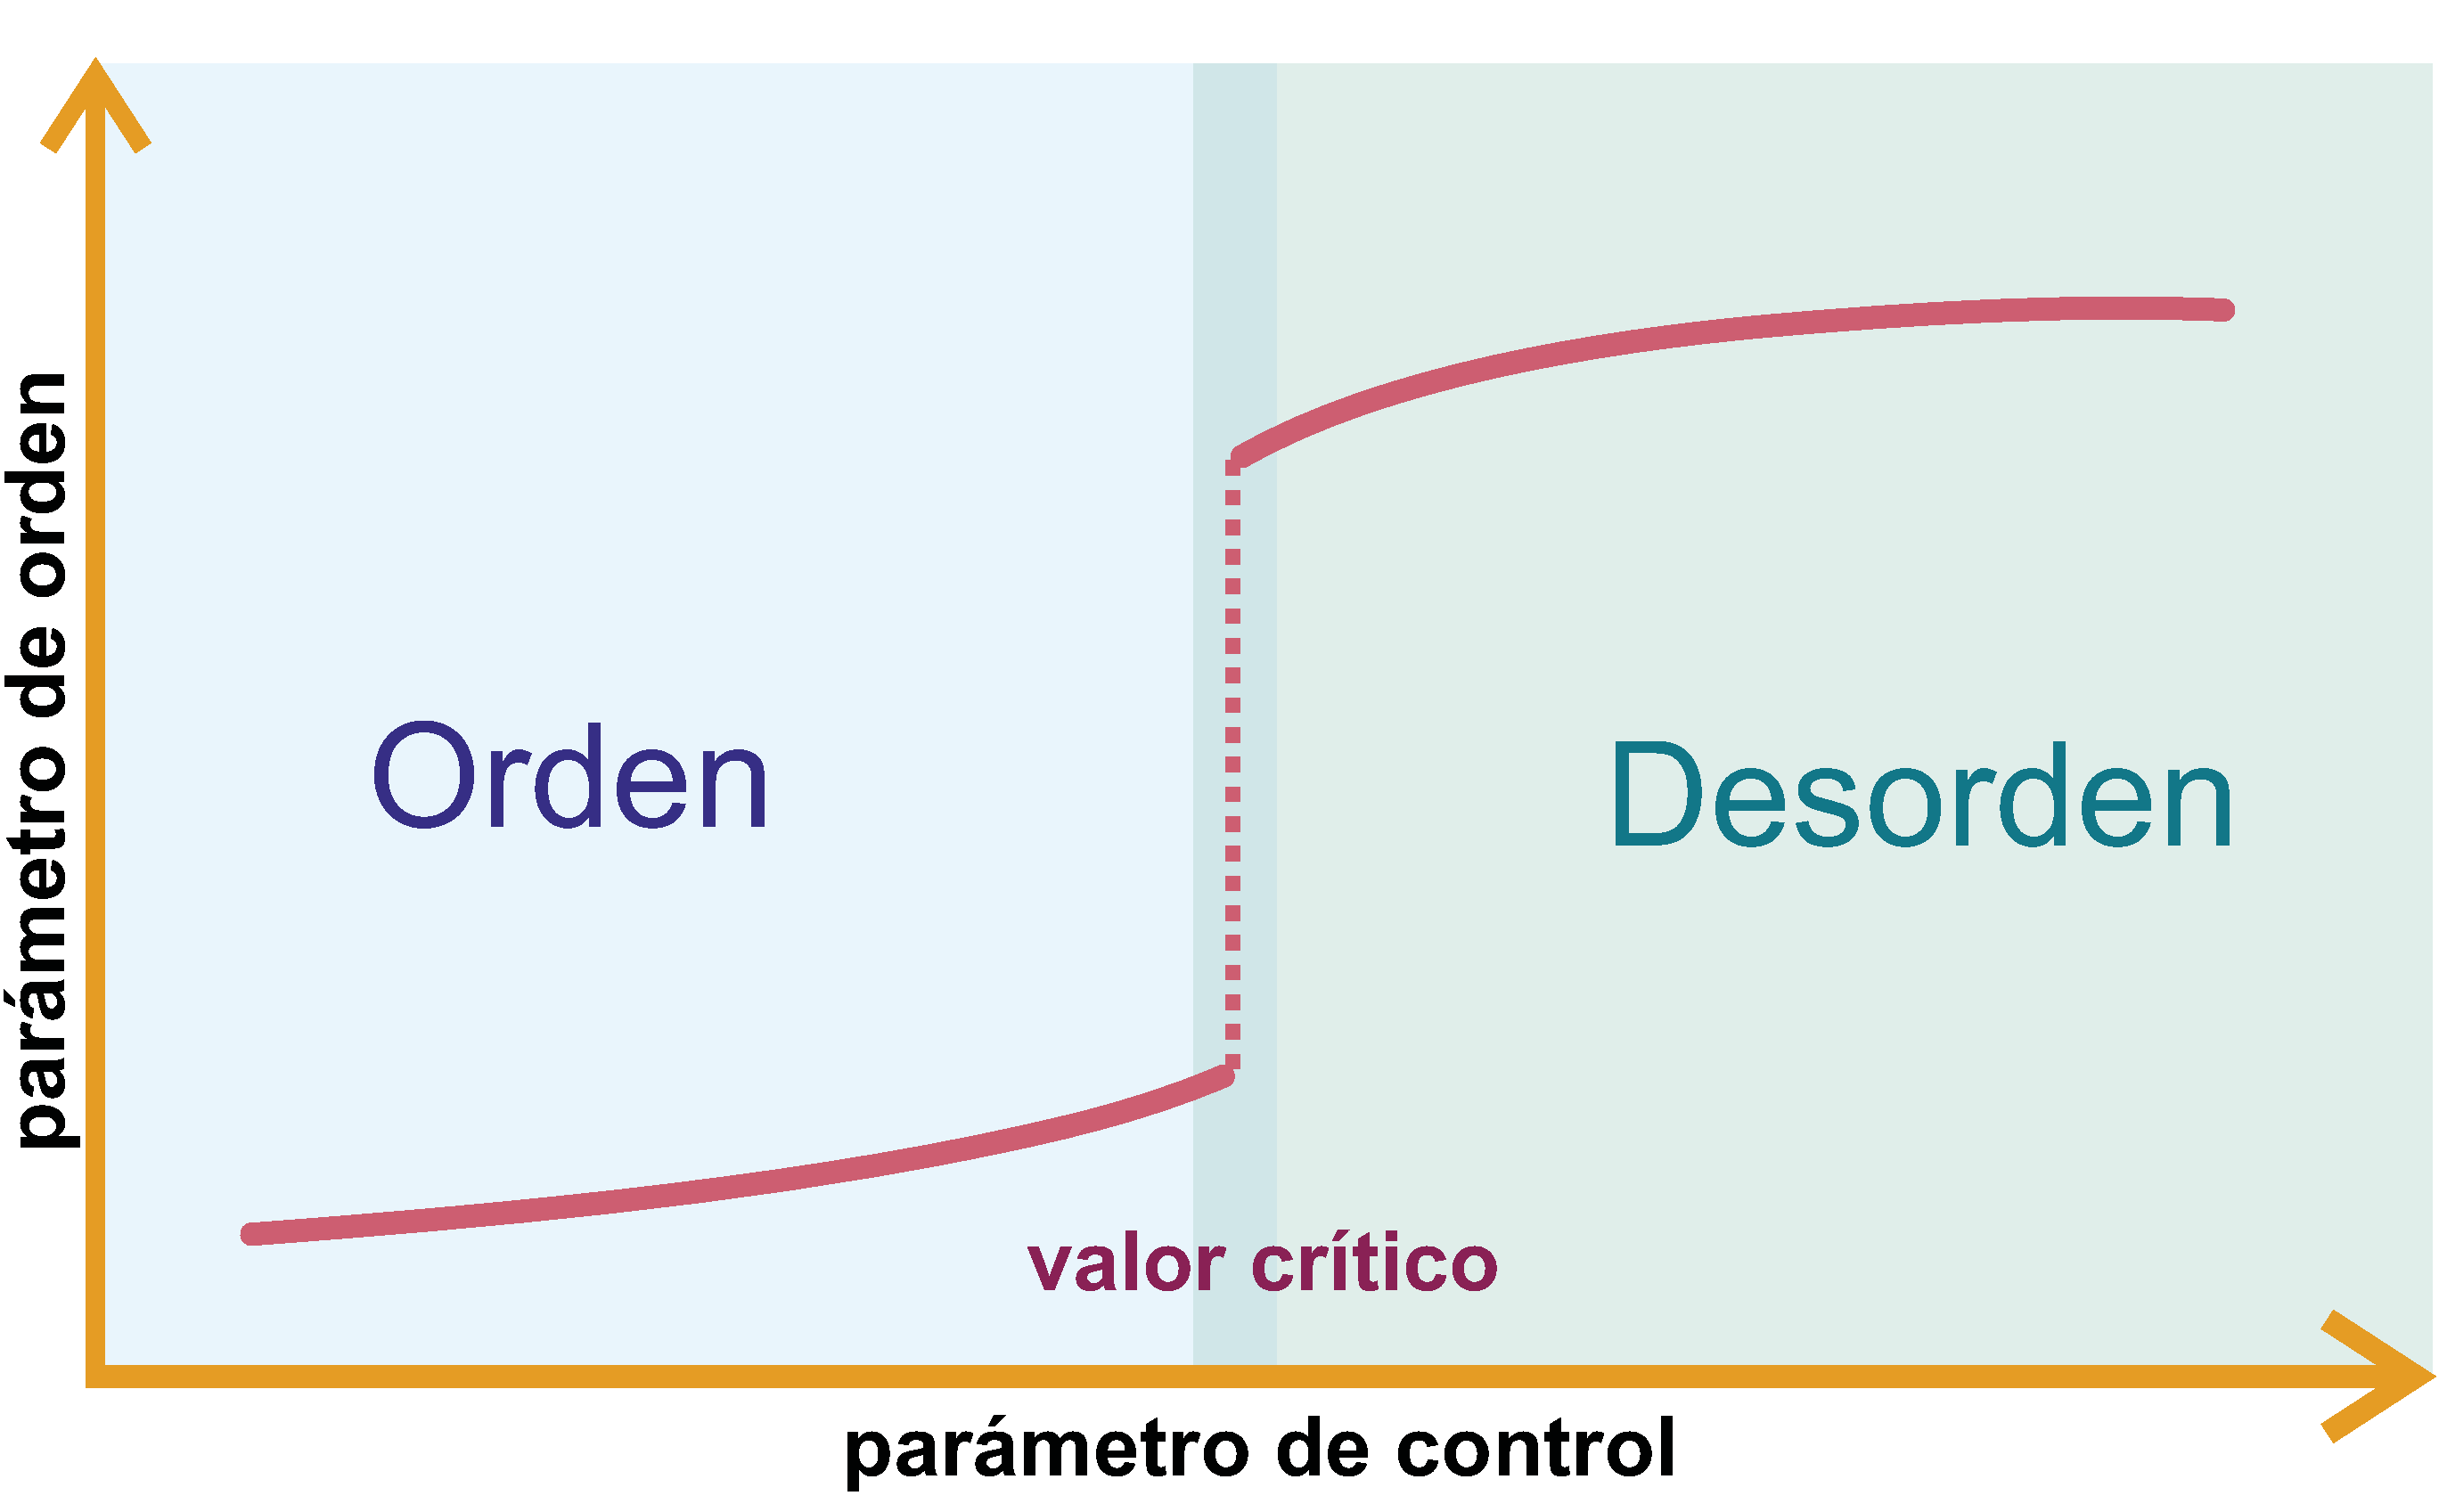
\includegraphics[width=\textwidth]{transiciones_fases_tipo_I.pdf}
		%\caption{transiciones de fase de primer orden}
		\caption{}
		\label{fig:transicionI}
	\end{subfigure}
	\begin{subfigure}[b]{0.45\textwidth}
		\centering
		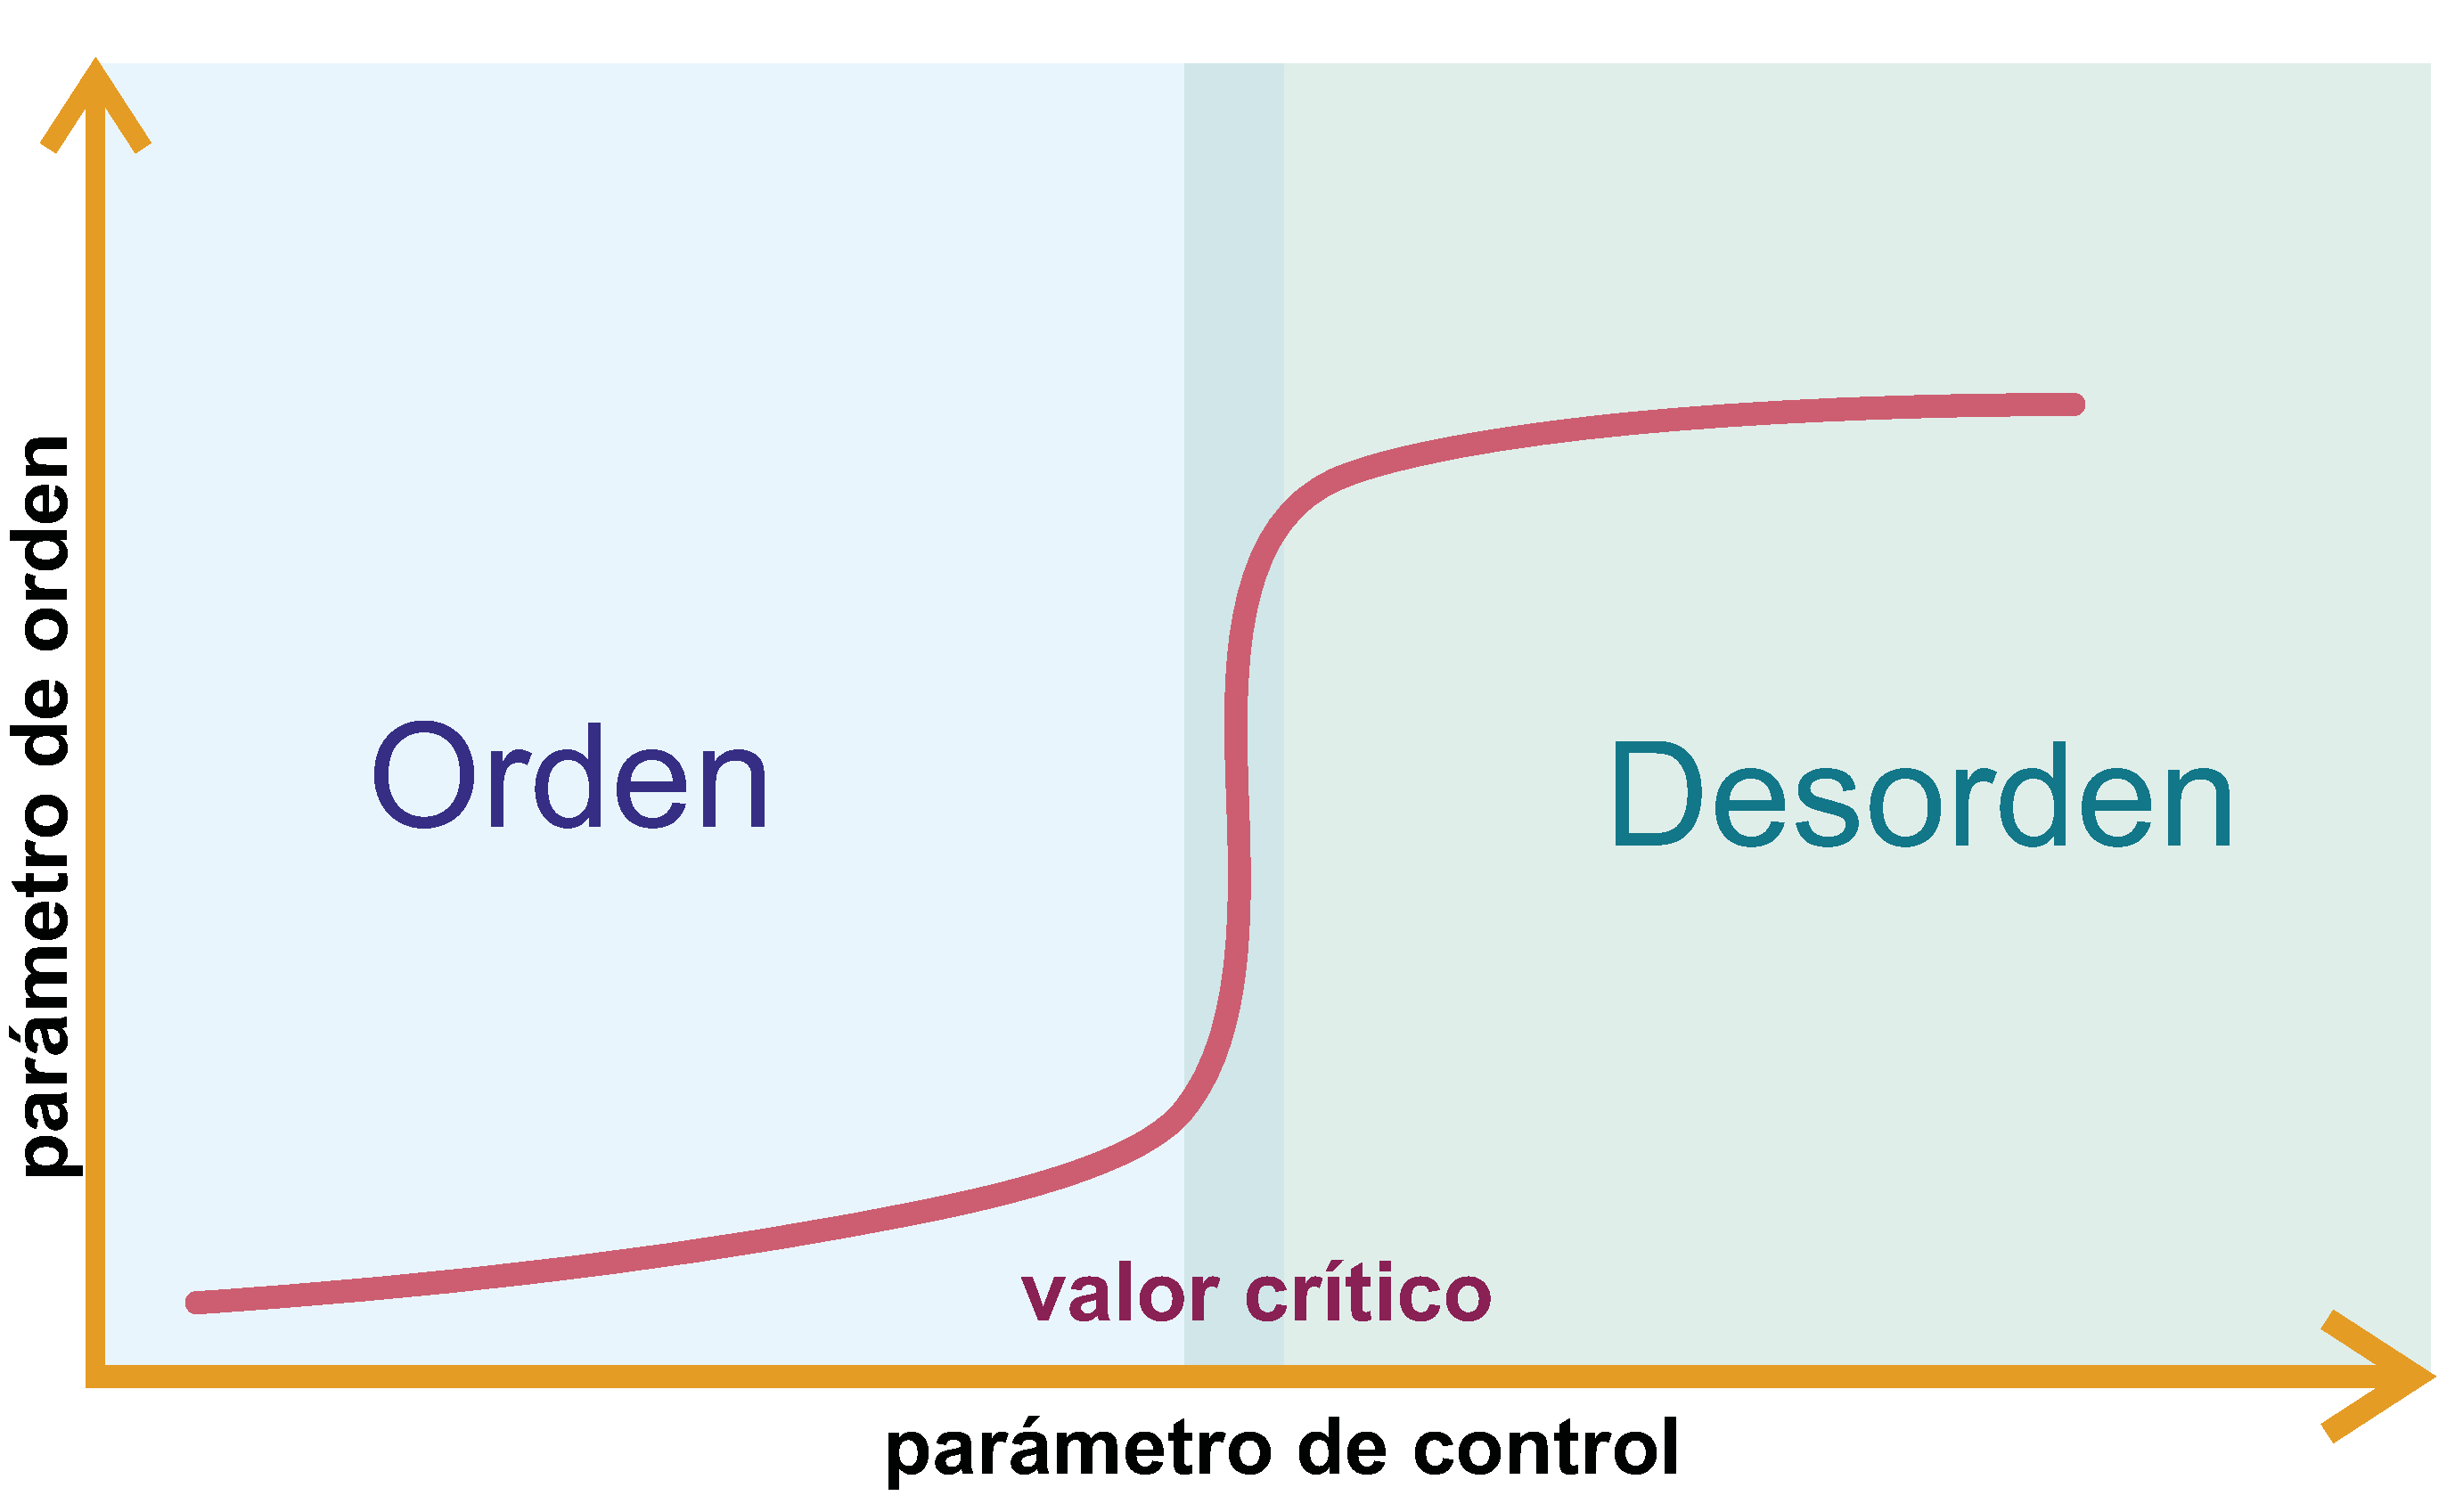
\includegraphics[width=\textwidth]{transiciones_fases_tipo_II.pdf}
		%\caption{transiciones de fase de segundo orden}
		\caption{}
		\label{fig:transicionII}
	\end{subfigure}
	\caption[Representaciones esquemáticas de transiciones de fase de primer y segundo orden.]{Representaciones esquemáticas de transiciones de fase de primer y segundo orden. La figura muestra dos ejemplos de transiciones de fase que ocurren en sistemas termodinámicos. En (a), se ilustra una transición de fase de primer orden, donde el parámetro de orden experimenta un cambio abrupto en su valor crítico del parámetro de control. En contraste, en (b) se muestra una transición de fase de segundo orden, donde el parámetro de orden varía suavemente a medida que cambia el parámetro de control.}
	\label{fig:trancisiones}
\end{figure}


\begin{figure}[ht]
	\centering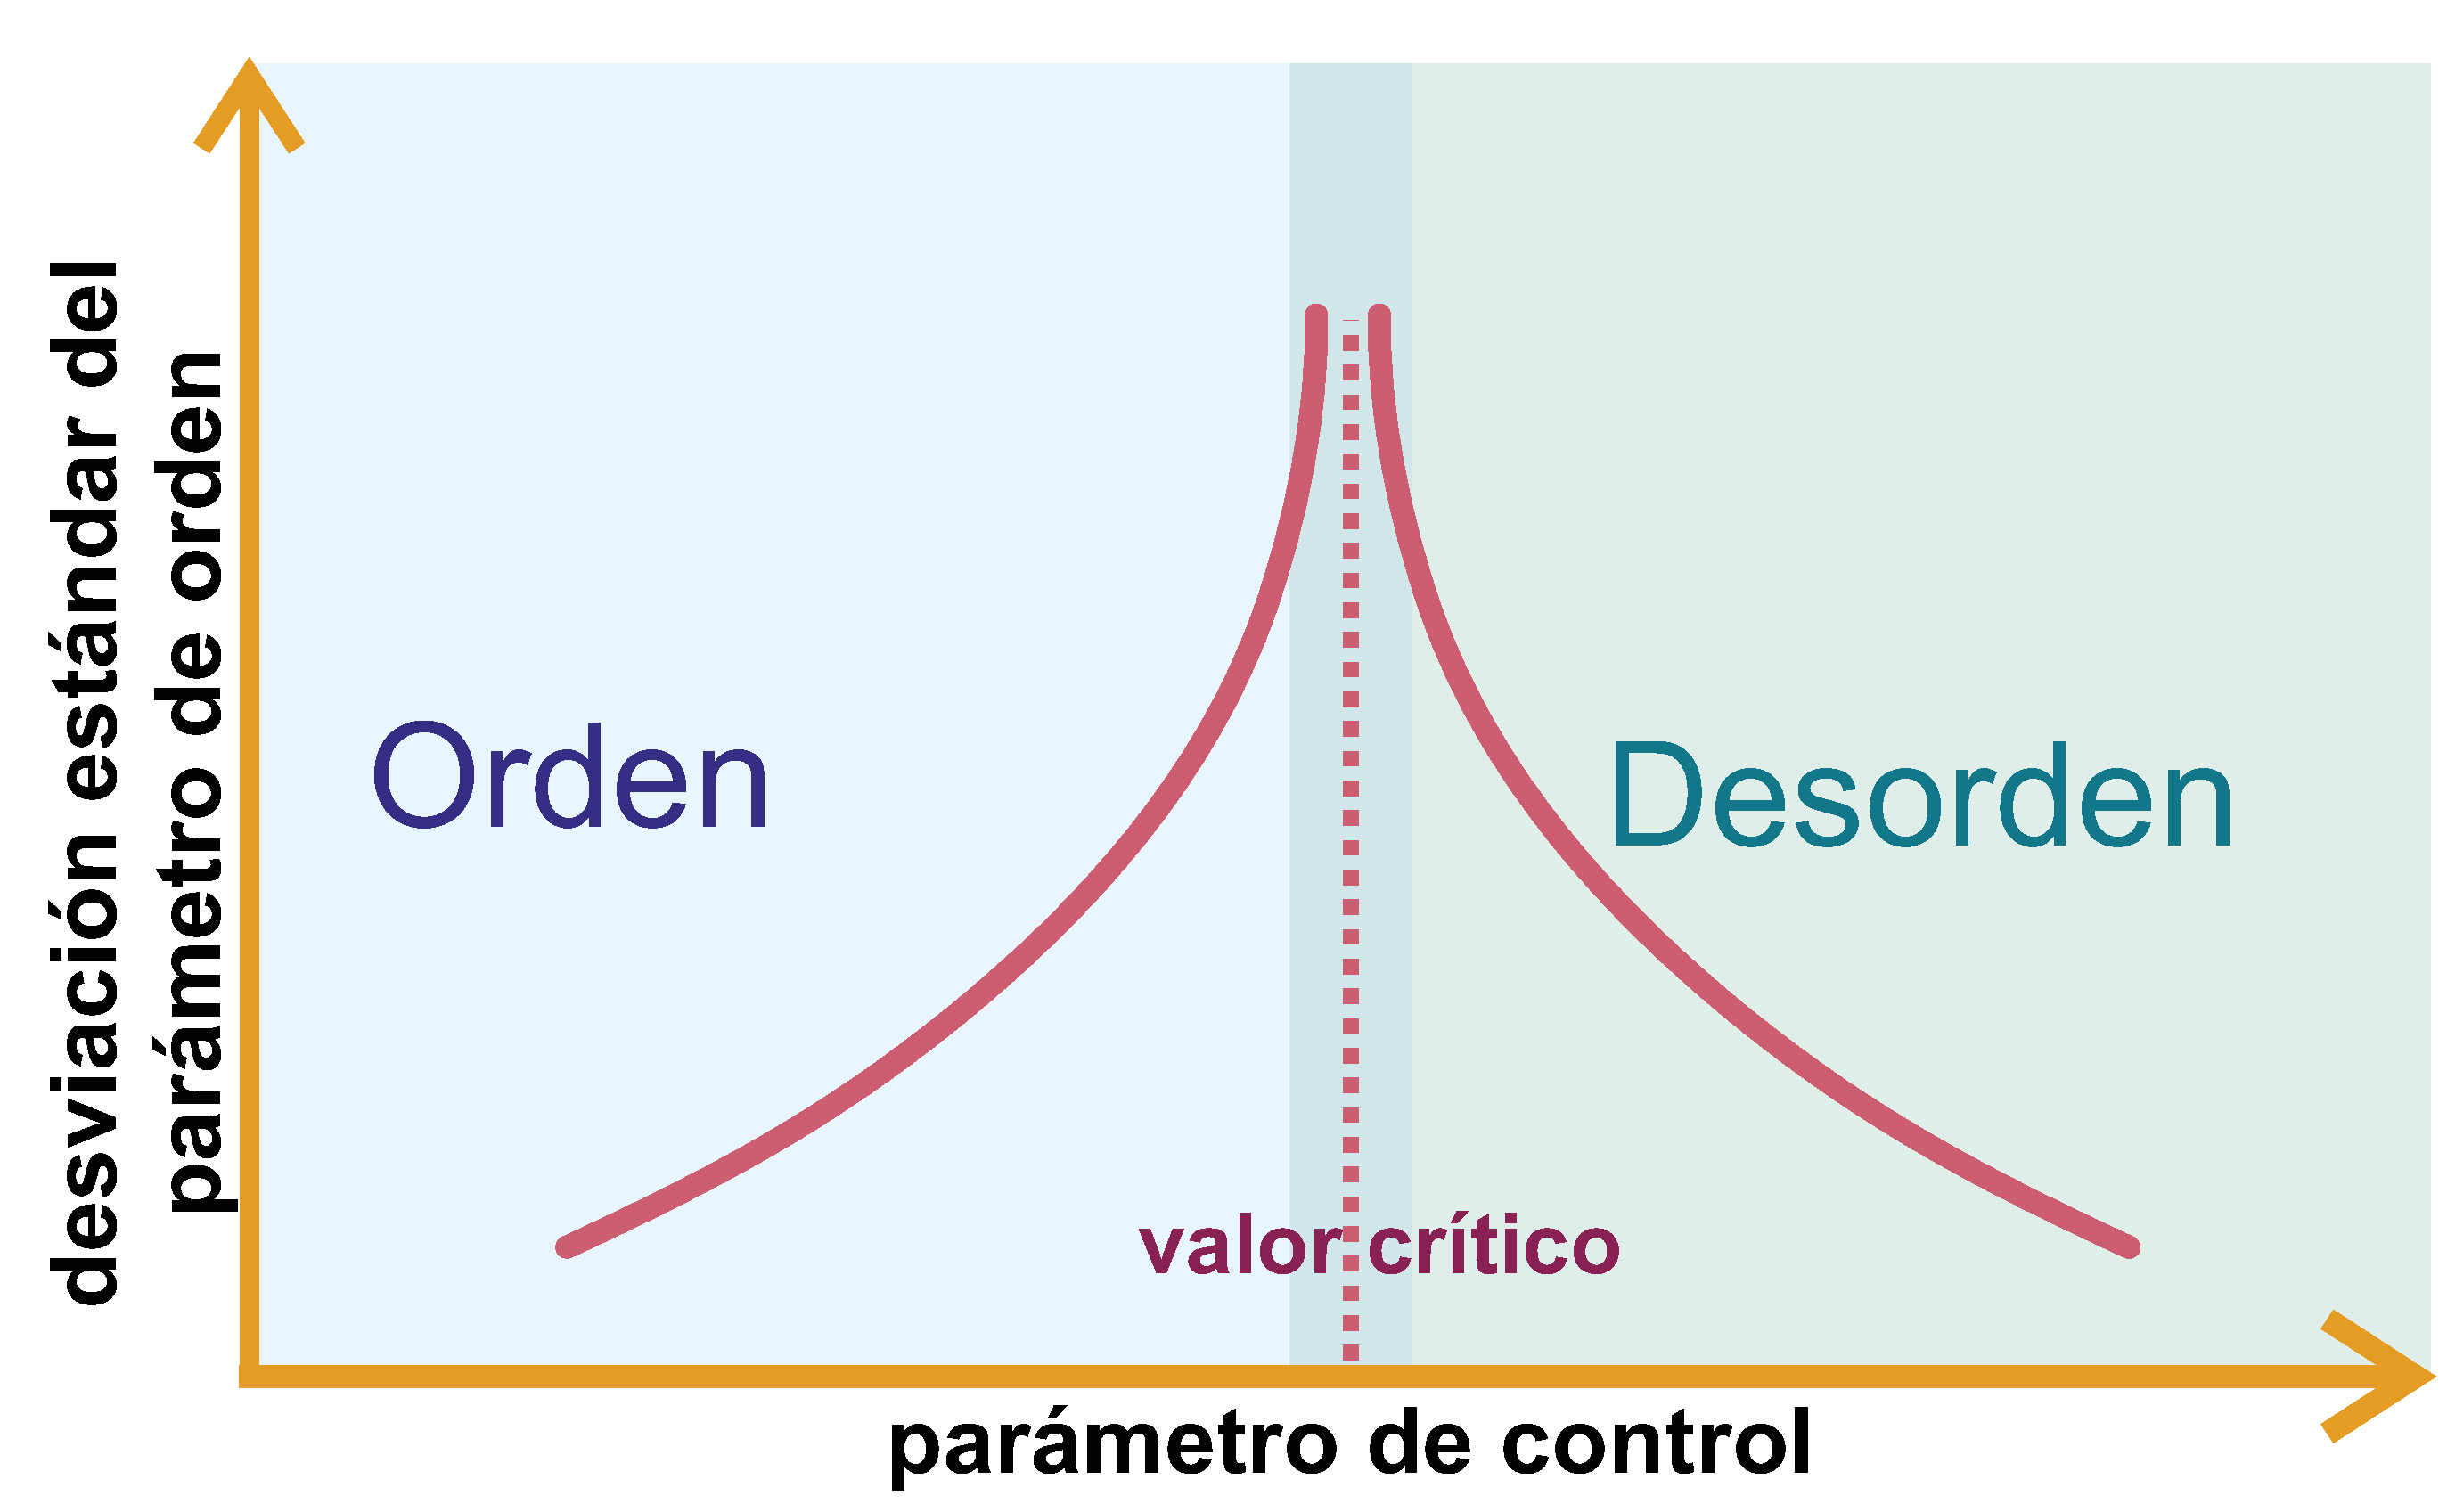
\includegraphics[width=\imsize]{transiciones_fases_tipo_II_divergencia}
	\caption[Desviación estándar del parámetro de orden en transiciones de fase crítica.]{Desviación estándar del parámetro de orden en transiciones de fase crítica. Durante las transiciones de fase crítica, se espera que el parámetro de orden exhiba fluctuaciones significativas. En particular, se observa un aumento en la amplitud de las fluctuaciones en el rango crítico, con la mayor desviación estándar en el valor crítico.} 	\label{fig:divergencia}
\end{figure}


Si un sistema exhibe una transición de fase continua, entonces puede existir en un punto crítico que se encuentra exactamente en la frontera entre dos fases distintas. Este estado límite, conocido como estado crítico, se caracteriza por la presencia de fluctuaciones importantes en el valor del parámetro de orden en el rango crítico, lo cual refleja la pérdida de simetría del sistema que ocurre durante las transiciones de fase. Por consiguiente, se considera que los estados críticos se encuentran en la frontera del caos. Las transiciones de fase críticas son especialmente interesantes debido al comportamiento crítico que se manifiesta en las grandes fluctuaciones del parámetro de orden, las cuales exhiben escalamiento de ley de potencia (Figura 1C).



\subsection{Transiciones de fase en biología}


El principio de universalidad es un concepto ampliamente aceptado en la física que establece que las características relevantes de los fenómenos a gran escala son altamente insensibles a los detalles específicos del modelo y se comparten entre sistemas aparentemente distintos. Siguiendo este principio, se ha propuesto una hipótesis controvertida, pero ampliamente investigada, según la cual algunos sistemas biológicos pueden obtener beneficios funcionales significativos al operar cerca del punto crítico de una transición de fase \cite{munoz_colloquium_2018,hidalgo_information-based_2014,kauffman_origins_1993,bak_how_1996,chialvo_brain_2008,chialvo_emergent_2010,plenz_critical_2013,niebur_criticality_2014,shew_functional_2013,cocchi_criticality_2017,zimmern_why_2020}. En particular, estos sistemas operarían en el límite entre una fase activa o caótica, en la que las fluctuaciones son amplificadas y la información se corrompe, y una fase inactiva u ordenada, en la que las fluctuaciones se amortiguan rápidamente y se reduce la capacidad de respuesta y adaptación. Se han identificado varios ejemplos de tales transiciones, como se resume en el \cref{table:transiciones_biologicas}.

% primer estilo 
%row{odd} = {bg=azure8},
%row{1} = {bg=azure3, fg=white, font=\sffamily},

% segundo estilo 

%row{odd} = {bg=red8},
%row{even} = {bg=red9},
%row{1} = {bg=red3, fg=white, font=\sffamily}

% tercer estilo 

%row{odd} = {bg=gray8},
%row{even} = {bg=gray9},
%row{1} = {bg=red3, fg=white, font=\sffamily},

%otra 

%row{odd} = {bg=teal9},
%row{1} = {bg=teal3, fg=white, font=\sffamily},
\begin{table}[h!]
	\centering
		\caption[Ejemplos seleccionados de transiciones de fase en biología.]{ Ejemplos seleccionados de transiciones de fase en biología, adaptado de Heffern et al\protect{\cite{heffern_phase_2021}}.}
\begin{tblr}{colspec={X[2,l]X[2,l]X[2,l]X[l]},
row{odd} = {bg=gray8},
row{even} = {bg=gray9},
row{1} = {bg=red3, fg=white, font=\sffamily},
}
	sistema	& parámetro de control	  &   parámetro de orden	& referencias seleccionadas\\
	  
	
	Fusión de la membrana plasmática	 & Temperatura	  &  Fluidez &    \cite{de_kruyff_effect_1972} \\
	

	Sincronización neuronal	 &   Fuerza sináptica; relación de excitación a inhibición	 &  Sincronización de tasas de disparo	 &    \cite{adhikari_time-delay-induced_2011,baumgarten_critical_2019}\\
	
	{Agrupamiento/enjambre}	 & Densidad; ruido en la percepción del comportamiento de los vecinos	  & Alineación de patrones de vuelo	  &   \cite{cavagna_scale-free_2010,bahar_flocking_2018,attanasi_finite-size_2014}  \\
	
	Rigidez de actina	 &   Densidad	 &   Rigidez &   \cite{gurmessa_triggered_2019,hussain_spatiotemporal_2013}  \\
	
Colapso de la población microbiana	 	&  Nivel de estrés	 & Crecimiento  &  \cite{mensonides_metabolic_2002,ordway_phase_2020}  \\
	
	Evolución cultural	 &  Cambios en el \gls{fitness} acompañado de \gls{epistasis} entre rasgos culturales	 &  Paradigma cultural	 & \cite{pascual_epistasis_2020}   \\ 
	
	
Rasgos del fitoplancton	 	& Condiciones de luz	  &   Contenido de clorofila	&  \cite{held_second-order_2020}  \\
	
	Colapso de la población de megafauna	 &   Variado& Tamaño de la poblacion	  &  \cite{hein_population_2019,lauerburg_socio-ecological_2020,heinze_quiet_2021}  \\ 
	
	Percolación de rigidez en embriogénesis de pez cebra	 &  Conectividad celular dependiente de la adhesión	 & Viscosidad del tejido, tamaño del grupo	  &  \cite{petridou_rigidity_2021}   \\
	
	\end{tblr}
	\label{table:transiciones_biologicas}
\end{table}

Existen varios experimentos que respaldan esta hipótesis. Algunos de estos ejemplos incluyen las transiciones de fase de sincronización en osciladores biológicos colectivos, como los relojes circadianos \cite{garcia-ojalvo_modeling_2004}; las transiciones de percolación de fibras en tejidos conectivos, como el colágeno \cite{forgacs_phase_1991,newman_phase_2004,alvarado_molecular_2013}; la transición de fase de fusión en hebras de ADN \cite{magee_jr_theory_1963,li_phase_2006}; las transiciones entre diferentes regímenes dinámicos, como las oscilaciones y los estallidos, en redes neuronales \cite{kelso_phase_1984,freeman_metastability_2005,rabinovich_dynamical_2006,werner_metastability_2007,adamatzky_chaos_2013,haken_principles_1996}; los patrones de expresión génica \cite{tsuchiya_self-organizing_2016};  el agrupamiento bacteriano \cite{larkin_signal_2018,ordway_phase_2020}  y la formación de colonias de C. elegans \cite{chen_c_2021}. Para obtener una revisión más completa de las aplicaciones de las transiciones de fase a problemas biológicos, se recomienda consultar la obra de Heffern et al \cite{heffern_phase_2021}.



\section{Hipótesis de la criticidad neuronal}
En línea con lo anteriormente expuesto, la hipótesis de la criticidad neuronal sostiene que el cerebro de los organismos puede estar en un estado crítico en el límite entre diferentes tipos de dinámicas \cite{hesse_self-organized_2014}.  De manera similar a lo que ocurre en los sistemas biológicos, se ha argumentado que la criticidad proporciona a los sistemas neuronales un equilibrio óptimo entre robustez frente a las perturbaciones y flexibilidad para adaptarse a condiciones cambiantes, así como para conferirles capacidades computacionales óptimas \cite{legenstein_edge_2007,tagliazucchi_signatures_2017}, amplios repertorios dinámicos \cite{shew_neuronal_2009}, gran estabilidad de la red \cite{bertschinger_real-time_2004}, transmisión y almacenamiento óptimo de la información \cite{plenz_organizing_2007,beggs_criticality_2007,haldeman_critical_2005,lombardi_balance_2012,vazquez-rodriguez_stochastic_2017}, máxima sensibilidad a los estímulos \cite{kinouchi_optimal_2006,liu_plasticity_2015}  y un comportamiento global coordinado \cite{schneidman_weak_2006,beggs_neuronal_2003}.

Numerosos modelos específicos, como redes booleanas \cite{kauffman_emergent_1984,derrida_random_1986}, máquinas de estado líquido \cite{langton_computation_1990}, redes neuronales y redes de filtración de nanopartículas de plata \cite{carstens_brain-like_2022} , han verificado esta hipótesis (ver también Haykin et al \cite{haykin_what_2007} para una revisión). 

Experimentalmente, se ha evidenciado que los sistemas neuronales parecen mostrar características de los sistemas en estado crítico, lo que sugiere que la hipótesis de la criticidad neuronal podría ser una explicación plausible para la dinámica del cerebro. Estos estudios incluyen:

\begin{itemize}
\item Invariancia de escala de las avalanchas neuronales \cite{fontenele_criticality_2019,beggs_neuronal_2003,beggs_neuronal_2004}  reportadas en diversas especies \cite{hahn_neuronal_2010,petermann_spontaneous_2009,shriki_neuronal_2013}, a través de diferentes técnicas de imagen \cite{tagliazucchi_criticality_2012} y señales electrofisiológicas \cite{linkenkaer-hansen_long-range_2001}. Al igual que en los sistemas biológicos, se ha encontrado que los sistemas neuronales exhiben una dinámica que es independiente de la escala temporal y espacial, lo que sugiere que los procesos neuronales son más similares a los procesos de los sistemas complejos en estado crítico que a los procesos aleatorios o regulares.
\item La presencia de correlaciones espacio-temporales de largo alcance en las fluctuaciones de amplitud de las oscilaciones neuronales \cite{expert_self-similar_2010,fraiman_what_2012,kitzbichler_broadband_2009}, incluida la observación de espectros de potencia $1/f$ de señales \acrshort{MEG}/\acrshort{EEG} registradas simultáneamente \cite{linkenkaer-hansen_long-range_2001}, resonancia magnética funcional  \cite{kitzbichler_broadband_2009} y respuestas cognitivas  \cite{van_orden_human_2005,shew_adaptation_2015}. Estas correlaciones sugieren que los sistemas neuronales exhiben una dinámica compleja y a largo plazo, lo que es consistente con la dinámica en estado crítico.
\item El aumento de la longitud de correlación con el tamaño del sistema \cite{fraiman_what_2012,ribeiro_trial-by-trial_2022,haimovici_brain_2013}. Al igual que en los sistemas biológicos, los sistemas neuronales parecen ser más estables y tener una dinámica más compleja a medida que aumenta el número de componentes.
\end{itemize}




\subsection{Mecanismos homeostáticos de mantenimiento  del estado Crítico}

Es posible conjeturar que la criticidad emerge en los sistemas vivos como resultado de procesos adaptativos y evolutivos que sirven como una plantilla para una mayor complejidad. Esta hipótesis propone que la criticidad podría ser una estrategia organizativa común en biología derivada de la física de las transiciones de fase. Sin embargo, aún hay muchas preguntas sin respuesta sobre la hipótesis de la criticidad.

Una de las principales preguntas es cómo un sistema complejo como el cerebro puede permanecer sintonizado en un estado crítico. Es importante tener en cuenta que la teoría de las transiciones de fase normalmente considera sistemas infinitos, mientras que en sistemas grandes pero finitos, las transiciones de fase se suavizan en un pequeño rango de parámetros. En lugar del punto crítico singular, encontramos una pequeña región que no es técnicamente crítica, pero que aún conserva muchas propiedades de criticidad \cite{moretti_griffiths_2013}. Sin embargo, incluso permanecer en esta región \textquote{crítica}  debería requerir mecanismos que resintonicen activamente el cerebro. La idea general de sistemas que se ajustan a estados críticos a través de procesos descentralizados activos se conoce como criticidad autoorganizada (\gls{soc}, por sus siglas en inglés) \cite{bak_how_1996,christensen_evolution_1998,bornholdt_topological_2000,bornholdt_self-organized_2003}.

El término \gls{soc}  describe las propiedades de los sistemas fuera del equilibrio para alcanzar un estado estacionario caracterizado por correlaciones de largo alcance, que se asemejan a las transiciones de fase de segundo orden cerca del equilibrio. En tales casos, el sistema desarrolla una respuesta multiescala que gradualmente alcanza un estado metaestable con correlaciones espaciales y temporales de largo alcance sin un parámetro de ajuste obvio o una transición de fase (dinámica). Por lo tanto, los estados del  \gls{soc} aparecen como un atractor de la dinámica no lineal en un sistema abierto repetidamente impulsado por fuerzas externas (o endógenas) \cite{tadic_self-organised_2021,gross_adaptive_2007}. 

Sin embargo, los sistemas nerviosos son sistemas no conservativos en contraste con los sistemas \gls{soc}  canónicos como los modelos de pilas de arena \cite{jensen_self-organized_1998,pruessner_self-organised_2012}. Para modelar tales sistemas, se utilizan redes no conservativas de elementos representados por autómatas celulares, mapas de tiempo discretos o ecuaciones diferenciales. Dichos modelos tienen características distintas de los sistemas conservadores. Una gran parte de ellos, en particular las redes neuronales, muestran \gls{SOqC} \cite{bonachela_self-organization_2009,bonachela_self-organization_2010,buendia_feedback_2020} o criticidad débil \cite{palmieri_emergence_2018,palmieri_forest_2020}. Con el tiempo, varios autores propusieron diferentes mecanismos biológicos que podrían eliminar el ajuste fino y convertir a la región crítica en un atractor autoorganizado \cite{kinouchi_mechanisms_2020,zeraati_self-organization_2021,meisel_adaptive_2009,droste_analytical_2013,tetzlaff_self-organized_2010,meisel_failure_2012,rocha_homeostatic_2018,plenz_self-organized_2021,levina_phase_2009,ma_cortical_2019}. La criticidad obtenida no es perfecta, pero es suficiente para dar cuenta de los datos experimentales. Además, los mecanismos (principalmente basados en sinapsis dinámicas, pero también en ganancias neuronales dinámicas, regulación homeostática de la inhibición y umbrales de activación adaptativos) son biológicamente plausibles y deben considerarse como un tema de investigación por derecho propio.


\section{Trastornos cerebrales y alteraciones de la criticidad}


En las anteriores secciones se ha examinado la relación de la criticidad con un comportamiento óptimo de la dinámica cerebral y los mecanismos que la organizan y mantienen. Se ha planteado la hipótesis de que las propiedades dinámicas que caracterizan un estado crítico pueden verse como un marcador importante del bienestar cerebral. En este sentido, las desviaciones de la criticidad pueden ser sintomáticas o causales de ciertas patologías, lo que allana el camino para nuevos diagnósticos y tratamientos.

A pesar del creciente interés en la criticidad biológica en las últimas dos décadas, ha habido una escasez de estudios experimentales y clínicos que conecten la criticidad con las perturbaciones. Debido a que la criticidad representa un estado óptimo para el cerebro, se esperaría que la salida del estado crítico suponga una interrupción en sí misma \cite{heiney_criticality_2021}. Sin embargo, en la práctica, las interrupciones en la dinámica de la red probablemente sean más complicadas que una transición fuera de la criticidad, ya que dichas transiciones pueden ser parte de una actividad saludable.

Es importante destacar que existen aplicaciones clínicas de estos hallazgos en varios trastornos neurológicos, como la epilepsia \cite{osorio_epileptic_2010,witton_rogue_2019,kramer_human_2012,moosavi_criticality_2023,meisel_antiepileptic_2020}, las enfermedades neurodegenerativas como la enfermedad de Alzheimer \cite{stam_disturbed_2005,montez_altered_2009,vysata_change_2014} y la enfermedad de Parkinson \cite{hohlefeld_long-range_2012,herrojo_ruiz_long-range_2014,west_parkinsonian_2016}, derrames cerebrales \cite{rocha_recovery_2022}, así como otros dominios clínicamente relevantes, como la anestesia \cite{alonso_dynamical_2014,thiery_long-range_2018,liu_scale-free_2014}, la medicina del sueño \cite{bocaccio_avalanche-like_2019} (incluyendo el insomnio \cite{meisel_decline_2017,colombo_more_2016}, la apnea del sueño \cite{lo_asymmetry_2013} y la narcolepsia), neurodesarrollo \cite{padilla_breakdown_2020,smit_scale-free_2011,mares_age-dependent_2013}, la cognición, atención, aprendizaje y autismo \cite{ezaki_closer_2020,jia_attenuation_2018,ouyang_decomposing_2020,tinker_power_2014,dimitriadis_altered_2013}, efectos psicológicos del neurofeedback y los psicodélicos \cite{zhigalov_modulation_2016,tagliazucchi_enhanced_2014}, las afecciones psiquiátricas comunes como la depresión \cite{gartner_aberrant_2017}, la esquizofrenia \cite{moran_long-range_2019}, la ansiedad \cite{tolkunov_power_2010} y el trastorno de estrés postraumático \cite{ros_tuning_2014}.  Se dispone de una revisión muy completa de estos temas en el artículo escrito por Vincent Zimmern \cite{zimmern_why_2020}.

No obstante, a pesar de los avances en la investigación, todavía no se ha incorporado la criticidad en la práctica clínica habitual. Esto se debe en parte a la falta de estudios experimentales y clínicos que conecten la criticidad con las perturbaciones, y también a la necesidad de formación de equipos multidisciplinarios en los que los físicos, matemáticos, científicos de datos y médicos colaboren para responder mejor a una pregunta clínica a través de la lente de la criticidad.

En este contexto, se espera que el futuro de la criticidad en el ámbito clínico dependa en gran medida de la formación de estos equipos multidisciplinarios y de la aplicación de técnicas de análisis cuantitativo de electroencefalografía (\gls{EEG}), \glossary{MEG} y resonancia magnética funcional (\gls{fMRI}), entre otras. De esta forma, podrían desarrollarse nuevas herramientas diagnósticas y terapéuticas que permitan una mejor comprensión y tratamiento de diversas enfermedades neurológicas y psiquiátricas.



\section{Métricas experimentales de criticidad}


En las secciones anteriores se ha presentado la hipótesis de criticidad y su relevancia en los sistemas biológicos, así como sus limitaciones y aplicaciones. En esta sección, se aborda la detección de las transiciones de fase y la dinámica crítica en experimentos y simulaciones.
La construcción de un diagrama de fase es la evidencia más directa de una transición de fase (ver \Cref{fig:trancisiones} ) \cite{dickman_paths_2000}. En este tipo de diagrama, se puede observar la respuesta del parámetro de orden ante las variaciones del parámetro de control, lo que permite detectar la existencia de una transición de fase. Sin embargo, la construcción de dicho diagrama requiere que el parámetro de control sea accesible y controlable en el entorno experimental, lo que puede resultar difícil en sistemas biológicos complejos.

Por ejemplo, la variación de la conectividad cerebral in vivo puede ser difícil de lograr experimentalmente. Debido a estas limitaciones, la mayor parte de la evidencia de la criticidad en sistemas biológicos proviene de la observación de características distintivas en los resultados experimentales. En esta sección, se discuten las características distintivas de la criticidad que se han identificado en la literatura científica y que se utilizan para establecer la presencia de criticidad en sistemas biológicos \cite{hesse_self-organized_2014}. Estas características distintivas son fundamentales para la identificación de la dinámica crítica en sistemas biológicos complejos, especialmente aquellos cuya dinámica interna es imposible o difícil  de modificar.



\subsection{Escalamiento de la ley de potencia}


En el ámbito de la estadística, una variable aleatoria continua $X$ se considera que tiene una distribución de ley de potencia cuando se extrae de una distribución de probabilidad con densidad $	\mathbb{P}\left(x\leq X\leq x+dx\right)=Cx^{-\alpha}dx$. El parámetro $\alpha$ se conoce como el exponente o parámetro de escala, mientras que $C$ es un parámetro de normalización. Por otro lado, una variable aleatoria discreta de ley de potencia tiene una versión discretizada similar de la probabilidad, que se puede expresar como 	$P(X=k)=Ck^{-\alpha}$.

Es importante señalar que en la práctica, son pocos los fenómenos empíricos que obedecen leyes de potencia para todos los valores de $X$. En general, las leyes de potencia se utilizan para caracterizar la cola de la distribución, es decir, la distribución de probabilidad de los valores de $X$ mayores que algún valor $x_{min}$. En estos casos, se dice que la cola de la distribución sigue una ley de potencia. Además, los datos a menudo muestran una distribución de ley de potencia truncada, lo que significa que el comportamiento de ley de potencia solo se observa en un rango limitado, $x_{min}\leq X \leq x_{max}$  \cite{touboul_can_2010}.

Cabe destacar que las leyes de potencia presentan invariancia de escala, lo que las convierte en distribuciones libres de escala. Una función $f(x)$ se considera invariante de escala si $ f(cx)  = \left(cx\right)^{-\alpha}=c^{-\alpha}x^{-\alpha}=c^{-\alpha}f(x)\propto f(x)$, lo que indica que escalar el argumento de la función es equivalente a escalar proporcionalmente la función misma. Además, como $\log(p(x))=\log_{\alpha}\left(ax^{-\alpha}\right) = -\alpha\log(x)+\log(a)$, el histograma de la ley de potencias presenta una relación afín en un gráfico logarítmico (\Cref{fig:leypotencia}).

Debido a esto, las leyes de potencia en datos empíricos se suelen analizar graficando el logaritmo del histograma en función del logaritmo de los valores de la variable aleatoria. Luego, se aplica un algoritmo de mínimos cuadrados para ajustar una línea afín a través de los puntos de datos. Este método se remonta a Pareto en el siglo XIX \cite{arnold_pareto_2008}. Sin embargo, es importante destacar que la inspección visual de un diagrama puede generar falsos positivos. Además, se ha señalado que las pruebas convencionales de bondad de ajuste no son adecuadas para las leyes de potencia \cite{newman_power_2005}.



\begin{figure}[ht]
	\centering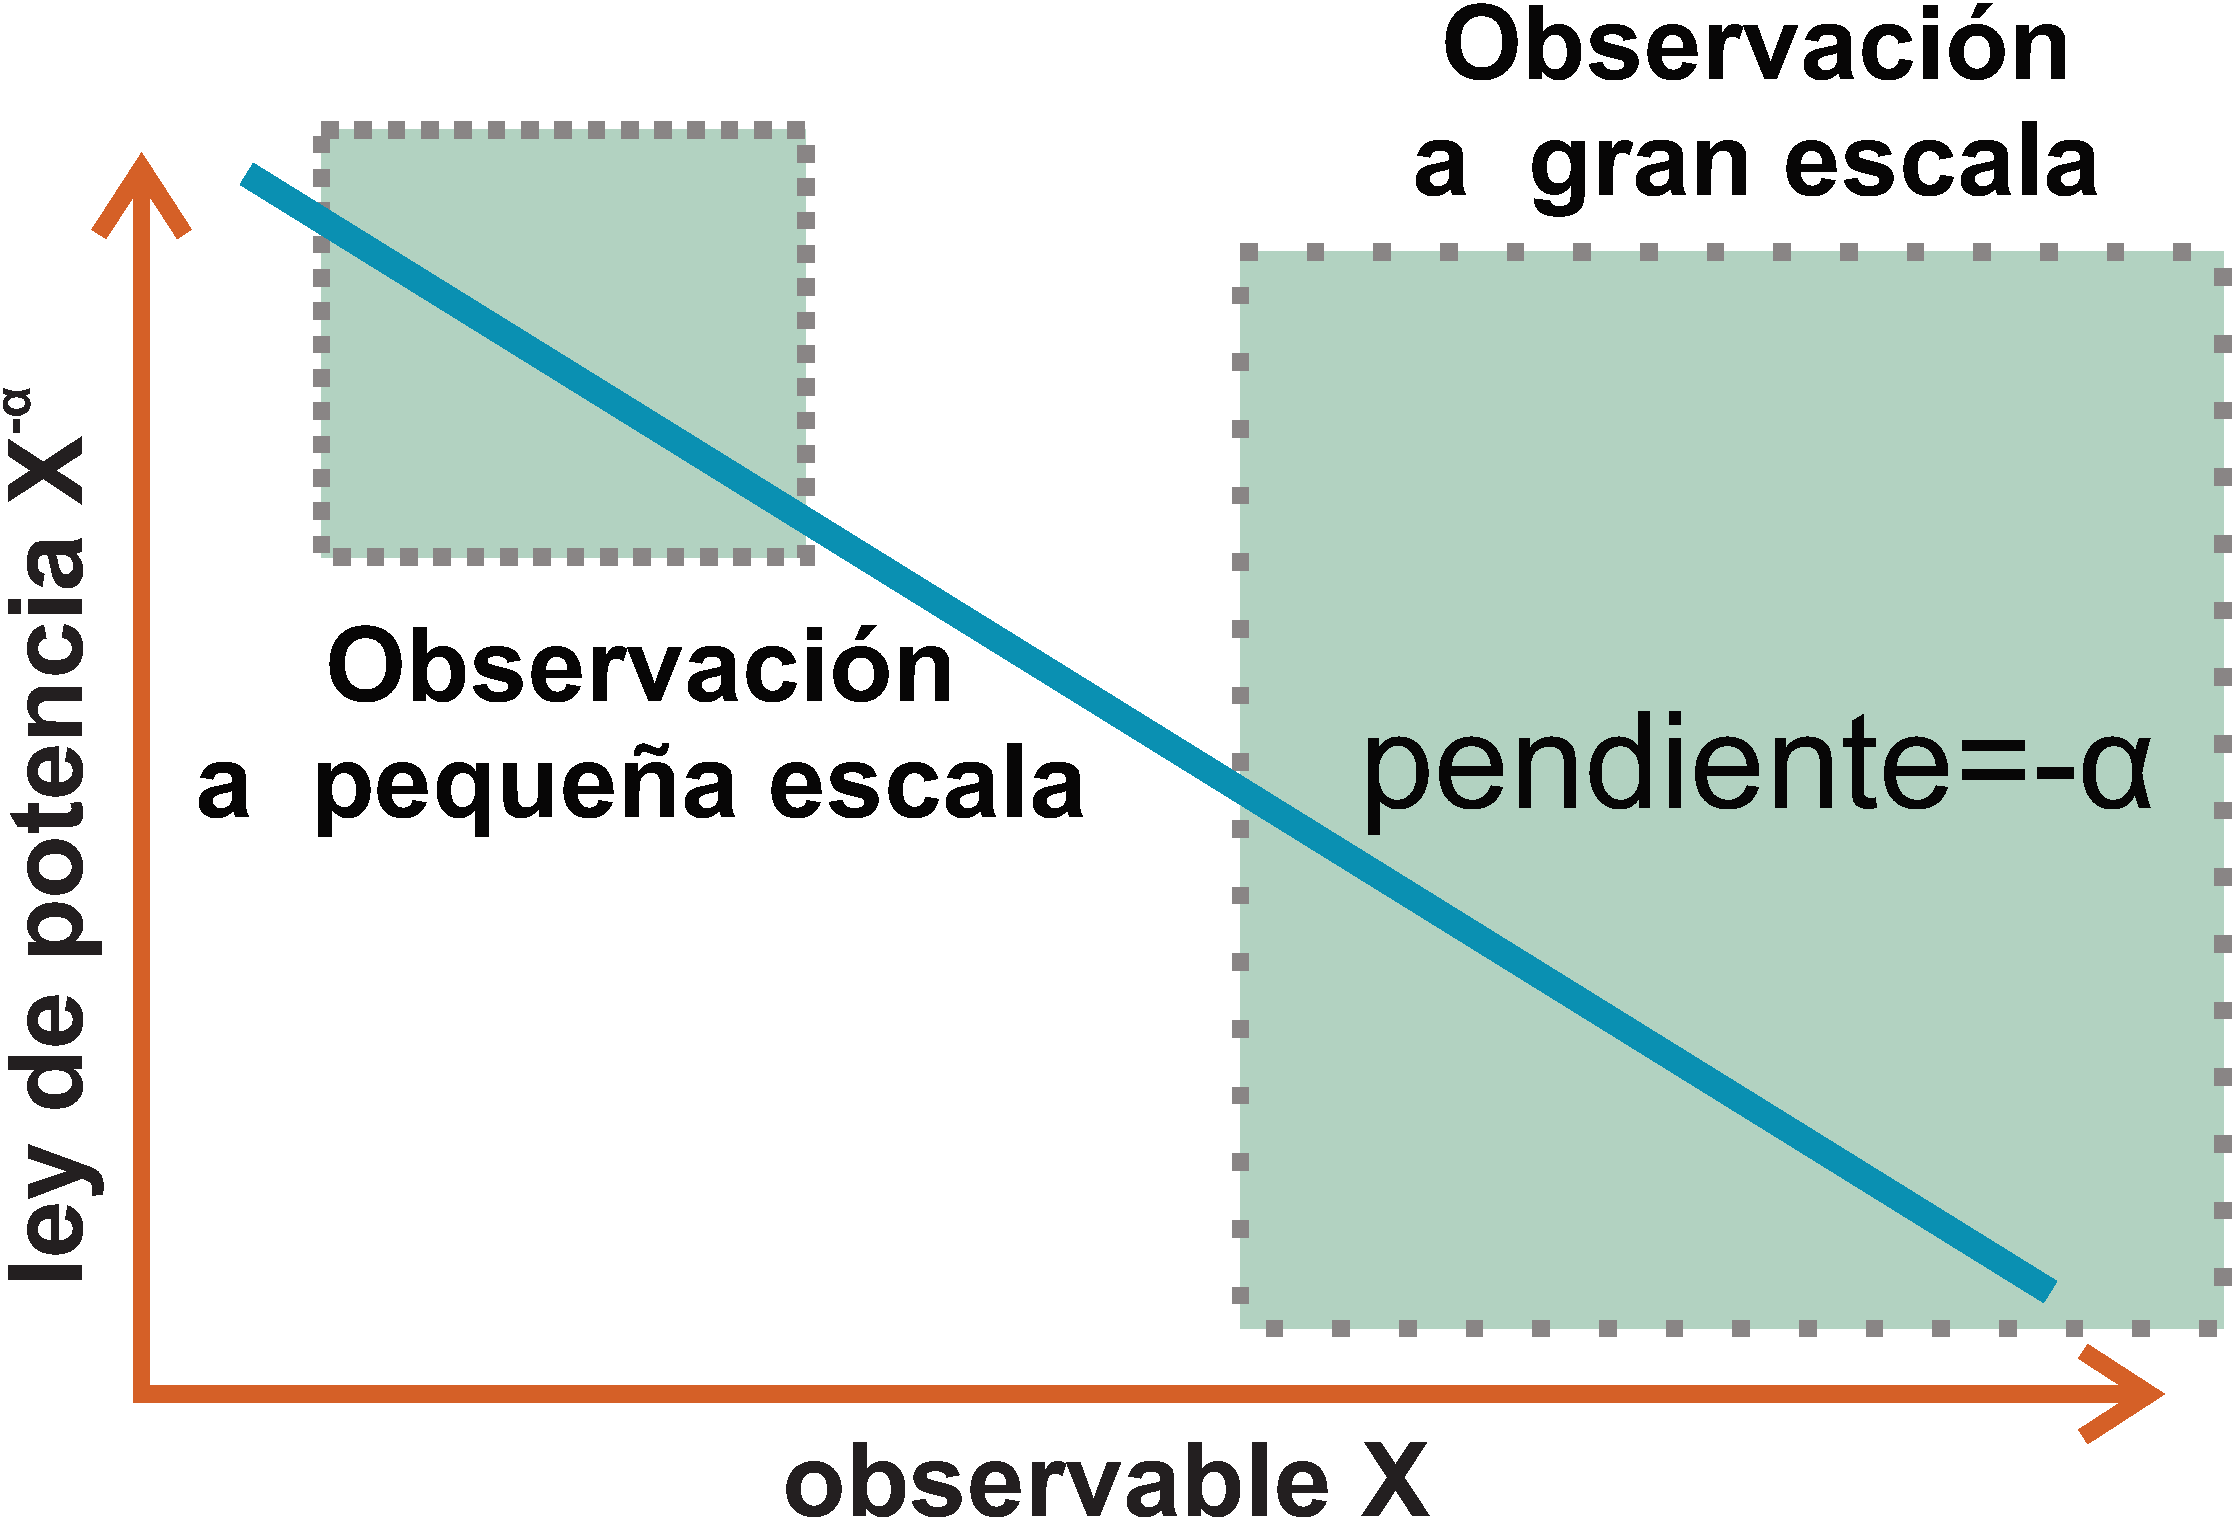
\includegraphics[width=\imsize]{ley_potencia}
	\caption[Representación gráfica de la independencia de escala de las leyes de potencia en una distribución de datos.]{Representación gráfica de la independencia de escala de las leyes de potencia en una distribución de datos, donde se ha utilizado la ley de potencia $f(x) = x^{-\alpha}$  con un exponente crítico de $\alpha=-1.5$ y una escala logarítmica en el eje $x$. La figura muestra que, independientemente del rango o escala utilizada para medir la distribución, se observa una ley de potencia con el mismo exponente crítico.} 	\label{fig:leypotencia}
\end{figure}


La hipótesis de criticidad en experimentos y simulaciones se basa en la presencia de leyes de potencia, que se espera se manifiesten en la mayoría de los sistemas críticos. Sin embargo, la existencia de leyes de potencia por sí sola no es suficiente para probar la criticidad \cite{goldstein_problems_2004,priesemann_can_2018}, ya que estas leyes también pueden ser explicadas por mecanismos no críticos \cite{touboul_can_2010,markovic_power_2014,noauthor_critical_2006,beggs_being_2012}. Por tanto, la identificación de leyes de potencia es un asunto delicado que requiere procedimientos de ajuste avanzados, debido a la dificultad para diferenciarlas de otras distribuciones de colas pesadas.

Las distribuciones de cola pesada son aquellas distribuciones de probabilidad cuyas colas son \textquote{más pesadas} que la distribución exponencial, siendo la gaussiana un subtipo de esta última. Entre los ejemplos de distribuciones de cola pesada se encuentran la distribución de Fisher-Tippett (doble exponencial), la distribución logarítmica normal y la distribución de Weibull, entre otras. Aunque se espera la presencia de leyes de potencia en sistemas críticos, estas distribuciones también pueden presentarse en otros sistemas no críticos. Por ende, para una mejor comprensión de la relevancia de las distribuciones de cola pesada en la neurociencia, se sugiere consultar la obra de Roberts et al  \cite{roberts_heavy_2015}.

Para abordar esta problemática, los investigadores han tenido acceso a metodologías estadísticas más sofisticadas gracias a los trabajos realizados por Clauset et al  \cite{clauset_power-law_2009} y otros estudios posteriores \cite{klaus_statistical_2011,markovic_power_2014}. Estas metodologías permiten distinguir las leyes de potencia de otras distribuciones de colas pesadas y evaluar su presencia en sistemas críticos. Sin embargo, es importante tener en cuenta que las leyes de potencia se truncan en sistemas de tamaño finito \cite{bonachela_self-organization_2010} y pueden verse afectadas por el submuestreo \cite{ribeiro_undersampled_2014}. Por lo tanto, es necesario emplear medidas cuantitativas para evaluar la diferencia entre las distribuciones de probabilidad acumulada experimental y ajustada por ejemplo  a través del parámetro $\kappa$ \cite{shew_neuronal_2009}.



\subsection{Escalamiento de  la ley de potencia de las avalanchas neuronales }

Beggs y Plenz demostraron experimentalmente que el comportamiento espontáneo de las redes corticales in vitro exhibe características consistentes con dinámicas críticas en su estudio histórico sobre avalanchas neuronales en cortes corticales interconectados con arreglos de microelectrodos (\gls{MEA}) \cite{beggs_neuronal_2003} . Una avalancha neuronal es una duración de actividad persistente que se propaga a través de la red y está marcada por períodos de silencio que preceden y siguen al período activo (ver \Cref{fig:avalancha}). En el caso de sistemas in vitro (es decir, cortes o cultivos disociados), la \textquote{actividad } puede referirse a los picos de mayor frecuencia o el \gls{LFP} de menor frecuencia, ya que se han estudiado ambas modalidades.

\begin{figure}[ht]
	\centering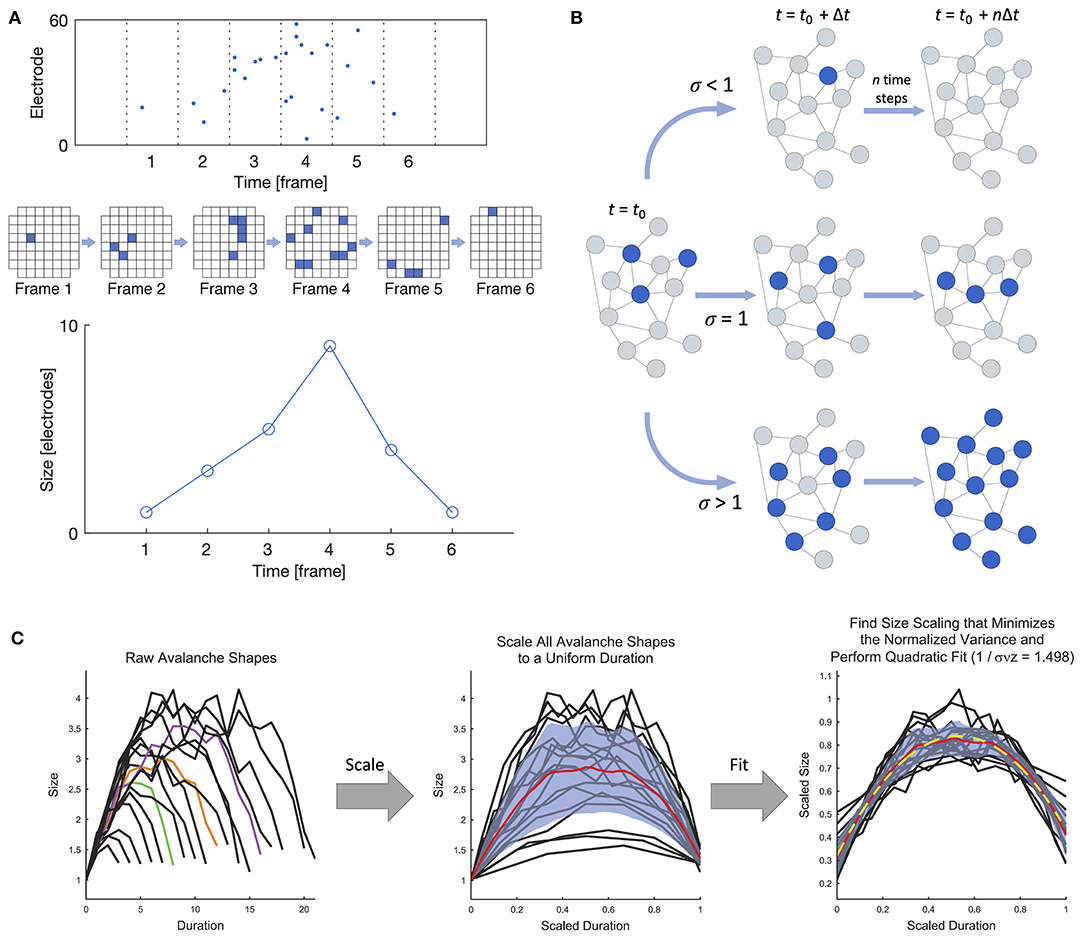
\includegraphics[width=\imsizeL]{fncom-15-611183-g002.jpg}
	\caption[Definición de avalancha neuronal y ejemplos de medidas empíricas de criticidad. ]{Definición de avalancha neuronal y ejemplos de medidas empíricas de criticidad. 
		(a) Se presenta la definición de avalancha neuronal, mostrando en el panel superior un gráfico rasterizado dividido en intervalos de tiempo. La avalancha representada abarca seis fotogramas activos, precedidos y seguidos por fotogramas inactivos. A continuación, se muestra una vista alternativa de la actividad en los seis marcos, en la que cada cuadrado representa un electrodo activo en una cuadrícula de 8x8. El panel inferior exhibe la definición de la forma de avalancha, la cual se obtiene a partir del número de electrodos activos en cada cuadro.
		(b) Se ilustra la relación de ramificación, en la cual los nodos azules representan actividad activa y los grises, inactiva. En una relación de ramificación de 1, la actividad persiste sin sobrecargar el sistema.
		(c) Se observa el colapso de forma en un sistema crítico, donde todas las avalanchas deberían mostrar el mismo perfil de forma temporal media en diferentes escalas de tamaño.
		Esta representación ha sido adaptada de Heiney et al.  \protect{\cite{heiney_criticality_2021}}.} 	\label{fig:avalancha}
\end{figure}


El escalamiento de la ley de potencia del tamaño $S$ y la duración $T$ de las avalanchas neuronales es un sello distintivo de la criticidad en las redes neuronales. Es decir, $P(S) \propto S^{-\alpha}$  y $P(T) \propto T^{-\beta}$, donde $P(\cdot)$  es la función de distribución de probabilidad. El tamaño se define generalmente como el número de electrodos o neuronas activados, y la duración es el número de intervalos de tiempo activos. Los exponentes de la ley de potencia del tamaño y la duración son aproximadamente $\alpha=1.5$ y $\beta= 2.0$, respectivamente, cuando se selecciona el ancho del intervalo de tiempo para que se corresponda con el intervalo promedio entre picos. Sin embargo, la escala de la ley de potencia debe persistir en un rango de resoluciones temporales cercano al orden de magnitud del intervalo promedio entre picos, con el exponente $\alpha$ cambiando sistemáticamente con el tamaño del intervalo de tiempo seleccionado \cite{beggs_neuronal_2003,pasquale_self-organization_2008}. La escala de ley de potencia también debe mantenerse cuando se considera una resolución espacial de grano más grueso, utilizando solo un subconjunto de todos los puntos de registro. Las redes neuronales pueden mostrar varios puntos críticos dinámicos únicos, de los cuales solo uno es la transición de fase que da lugar a las avalanchas neuronales. Por lo tanto, es crucial considerar el contexto más amplio y no limitarse a la transición de fase en sí misma \cite{kanders_avalanche_2017}.







\subsection{Parámetro de ramificación}



En la teoría de los procesos de ramificación \cite{harris_theory_1963} se utiliza una medida común, la relación de ramificación $\sigma$, para evaluar el número de descendientes y ancestros en un sistema. En particular, esta medida establece la proporción entre el número de descendientes y el número de ancestros, en el que la actividad en un electrodo o neurona ancestro precede inmediatamente a la actividad en un electrodo o neurona descendiente \cite{beggs_neuronal_2003}. En un sistema en estado crítico, la relación de ramificación se aproxima a $1$, lo que permite que la actividad fluya a través de la red sin extinguirse ($\sigma < 1$) o saturar toda la red ($\sigma > 1$), tal como se muestra en la \cref{fig:avalancha}. Por tanto, la presencia de una relación de ramificación $\sigma = 1$ en respuesta a una excitación artificial en un sistema lo suficientemente inactivo puede considerarse como una evidencia de criticidad.

No obstante, es importante destacar que, en comparación con otras características, la evidencia proporcionada por una relación de ramificación de uno es relativamente débil. Esto se debe a que dicha relación no implica necesariamente una dinámica crítica, ya que también puede ser observada en estados supercríticos \cite{hesse_self-organized_2014}. Por lo tanto, se requiere de un análisis más riguroso que permita distinguir entre ambos estados.


\subsection{Colapso de forma}


La dinámica de los sistemas críticos se caracteriza por la presencia de avalanchas de actividad, que exhiben una naturaleza autosimilar o fractal. Se espera que la \textquote{forma} de la actividad de la avalancha se comporte como un fractal en dichos sistemas. En un estado crítico, se espera que todas las avalanchas muestren el mismo perfil temporal medio en todas las escalas. El perfil temporal de una avalancha se define como el número de sitios activos en función del tiempo. Para un sistema en estado crítico, los perfiles temporales de todas las avalanchas colapsan en la misma forma de perfil cuando se escala espacio-temporalmente con un exponente de escala$\gamma$ cercano a $2$(\Cref{fig:avalancha}). Esta propiedad se describe por  $ \left\langle S\right\rangle(T) \propto T^{-\gamma}$, donde $\left\langle S\right\rangle(T)$  representa el tamaño promedio de todas las avalanchas de una duración determinada $T$.

Se puede encontrar información detallada sobre el colapso de la forma en la literatura científica, como en Sethna et al \cite{sethna_crackling_2001} y Friedman et al \cite{friedman_universal_2012}. Además, Miller et al \cite{miller_scale-invariant_2019} proporciona una demostración experimental del colapso de la forma en primates no humanos. El coeficiente de criticidad (DCC) de Ma et al \cite{ma_cortical_2019} se relaciona con el concepto de colapso de forma y se calcula a partir de la diferencia entre el exponente de escala $\gamma$, obtenido a partir de datos empíricos mediante regresión lineal, y el valor esperado obtenido a partir del exponente de ley de potencia $\alpha$ de la distribución de tamaños.


\subsection{Submuestreo espacial}

Debido a la naturaleza intrínseca de la observación de los sistemas neuronales, se ve limitada la capacidad de muestrear todos los componentes del sistema. Como consecuencia, se puede obtener únicamente una muestra espacialmente submuestreada del sistema, la cual puede resultar insuficiente para obtener conclusiones precisas acerca de la dinámica subyacente del sistema. Para abordar este problema, se han desarrollado métodos que involucran el escalado del submuestreo espacial \cite{levina_subsampling_2017} y el uso de un estimador invariante de submuestreo \cite{wilting_inferring_2018}. Estos métodos permiten la evaluación precisa de los estados dinámicos de sistemas submuestreados, incluso en situaciones donde el número de componentes muestreados es significativamente menor que el número total de componentes del sistema.



\subsection{Correlación temporal de largo alcance, ralentización crítica y flickering}


En sistemas críticos, la respuesta del sistema a los estímulos externos se maximiza, lo que se conoce como rango dinámico o correlación dinámica. La criticidad del sistema genera retornos geométricos al estado estacionario \cite{hesse_self-organized_2014}, lo que resulta en una correlación temporal de largo alcance \gls{LRTC} o memoria larga. La \gls{LRTC} puede medirse de diversas maneras, siendo los métodos más populares el exponente de Hurst, a través de varios estimadores, y   \gls{DFA}  \cite{hardstone_detrended_2012}. Este último produce un exponente de escala durante un período de tiempo determinado. Un exponente de escala entre $0.5$ y $1$, con un buen ajuste, indica que la serie de tiempo exhibe \gls{LRTC} durante ese período.

La tasa geométrica de retorno al estado estacionario también se conoce como desaceleración crítica \cite{scheffer_early-warning_2009}. En el punto crítico, la correlación dinámica del sistema diverge de tal manera que se producen avalanchas, es decir, actividad de la red, en todas las escalas del sistema \cite{hesse_self-organized_2014}. Este fenómeno se debe a que la fluctuación en la criticidad del sistema se propaga a través de la red, generando actividad a diferentes escalas. Además, en la transición crítica, surge el fenómeno del flickering, que se produce cuando el ruido permite que un sistema migre de un lado a otro entre dos cuencas atractoras \cite{wang_flickering_2012}. En este caso, el sistema se encuentra en un estado metaestable y su comportamiento no puede ser descrito por un solo atractor.




\subsection{Ruido $(1/ f )$ y ley de potencia}

Los sistemas críticos exhiben respuestas geométricas superpuestas a entradas débiles, lo que produce ruido $1/f$, también conocido como ruido rosa, ruido de ley de potencia o ruido flicker. La dependencia de largo alcance o memoria larga se utiliza a menudo como sinónimo de estos términos, ya que se trata de fenómenos idénticos. El término ruido $1/f$ se refiere al espectro de potencia $S(f)$ de una serie temporal, el cual sigue una ley de potencia de la forma $S( f ) = \alpha f^{-\beta}$. Históricamente, se han identificado los casos $\beta=0$, $\beta=1$, $\beta=2$ como ruido \textquote{blanco}, ruido \textquote{rosa}  y ruido \textquote{marrón}, respectivamente \cite{li_fractal_2005}. El ruido $1/f$ se acepta comúnmente en el rango  $0.5 < \beta < 1.5$. Si bien todos los sistemas críticos deben exhibir ruido $1/f$, no todo el ruido $1/f$ es indicativo de criticidad \cite{bedard_does_2006,hesse_self-organized_2014}. 



\section{Discusión}

La hipótesis de la criticidad neuronal está motivada por la relación entre la criticidad y las propiedades computacionales óptimas. La hipótesis está respaldada por experimentos que observaron características de criticidad para una amplia gama de animales, en varios estados de conciencia y en muchas escalas experimentales diferentes, desde grabaciones de unas pocas neuronas hasta todo el cerebro.  Sin embargo, se ha señalado que algunas pruebas pueden ser engañosas \cite{clauset_power-law_2009} y podrían explicarse potencialmente por mecanismos alternativos \cite{botcharova_power-law_2012,galinsky_neuronal_2023}. Algunos estudios experimentales también informan resultados negativos donde no se observaron características de criticidad en la actividad neuronal  \cite{yu_scale-invariant_2014,bedard_does_2006,dehghani_avalanche_2012}. En general, la relación entre el marco teórico y su realización biológica sigue sin estar clara.  Con base con lo presentando en este capitulo , consideramos que la criticidad es preferible a las explicaciones alternativas porque proporciona una explicación motivada por la evolución para varias observaciones que de otro modo estarían desconectadas.

A pesar de las advertencias antes mencionadas, la creciente investigación empírica y de modelado respalda claramente la opinión de que la dinámica neuronal probablemente ocurra cerca de inestabilidades críticas. El reconocimiento de las limitaciones de este nuevo campo simplemente muestra que ha madurado más allá de las primeras etapas. El objetivo principal de este capitulo fue el de realizar una revisión de la relevancia, limitaciones y aplicaciones de la hipótesis de criticidad neuronal.   En la mayor parte de estas investigaciones tanto en los experimento  como en  el modelado  la criticidad fue analizada a nivel \textquote{macroscópico} es decir en grandes regiones del cerebro particularmente en la corteza cerebral.  Desafortunadamente no existen experimentos que analicen la criticidad neuronal a nivel de todo el sistema nervioso de un organismo. Esto en parte es debido a que las técnicas que realizan  un seguimiento de la actividad neuronal de todo el sistema nervioso  son  recientes y están limitadas a organismos simples como por ejemplo el C. elegans \cite{kato_global_2015,kaplan_nested_2020,yemini_neuropal_2021}. Otro inconveniente es que aun teniendo toda la dinámica neuronal global  de un organismo esta debe modificarse  mediante fármacos, manipulación genética u otras técnicas para verificar que el estado optimo es el cercano al estado critico, por lo que muchos animales deben utilizarse y adaptar varios protocolos experimentales a estos cambios. Por otro lado los modelos que analizan la dinámica  critica  con el  conectoma completo del C. elegans son escasos  \cite{ciftci_synaptic_2018} y ninguno de ellos  analiza la dinámica critica de todo el sistema nervioso en ausencia de estímulos y los contrasta con resultados experimentales.

Sabiendo las limitaciones experimentales y los pocos modelos que analizan la dinámica critica a nivel global esta parte de la tesis busca  aportar  a estas limitaciones proponiendo una solución a la pregunta ¿Existe una dinámica critica a nivel global en el C. elgans  en ausencia de estímulos
externos?. Para responder a esta pregunta  en primer lugar  se aplicaran  algunas de las métricas experimentales de criticidad presentadas en este capitulo  en  datos experimentales de la dinámica neuronal global de  gusanos inmovilizados suministrados por (Kato et al) \cite{kato_global_2015}, (Kaplan et al)  \cite{kaplan_nested_2020} y neuropal \cite{yemini_neuropal_2021}.  El  objetivo especifico es analizar en que región se encuentra los datos experimentales de las   dinámicas neuronales del C. elgans.  Nuestra hipótesis de trabajo es que aun en un organismo tan pequeño como lo es el C. elegans la dinámica neuronal se encuentran en un régimen dinámico cercano al punto crítico de una transición de fase de segundo orden.


Por otro lado para superar las limitaciones experimentales de no poder manipular en tiempo real la dinámica neuronal y  tener un mayor control de los parámetros del sistema se plantea un modelo utilizando  el Conectoma  realizado por Cook y coautores  \cite{cook_whole-animal_2019} el cual abarca  todas las conexiones  neuronales  del C. elegans  junto a una  dinámica neuronal descrita por una regla dinámica no lineal muy simple la cual es una  adaptación del modelo neural Greenberg-Hastings introducida por Haimovici y coautores  \cite{haimovici_brain_2013}.   El  objetivo específico busca cuantificar la dinámica critica  en términos de un parámetro de orden   que emerge al manipular tanto los parámetros de  la dinámica neuronal  como el parámetro de control del sistema.  La hipótesis de trabajo es que los patrones espacio temporales observados de manera experimental en la actividad cerebral en ausencia de estímulos  solo pueden ser descriptos por un modelo de red neural si la misma se encuentra en un estado crítico. Finalmente, como objetivo específico buscaremos establecer relaciones entre los resultados experimentales y  nuestro modelo. En el siguiente capitulo se introducirá  mediante la teoría de percolaciones  el parámetro de orden que  nos permitirá caracterizar la transición de fase que surge al aplicar una dinámica critica al conectoma del C. elegans. 



% o cual se denomina la condición del estado de reposo.  Esta actividad espontánea se organiza en patrones espaciales bien establecidos llamados Redes del estado de reposo (Resting State Networks, RSN).  Las RSNs están formados por regiones del cerebro que están altamente correlacionadas en promedio, pero fluctúan en el tiempo y formando un repertorio de los estados metaestables.  Estudios anteriores mostraron  que las RSNs tienen propiedades que  recuerdan a los sistemas termodinámicos que experimentan una transición de fase de segundo orden y, por lo tanto, respaldan la hipótesis de que el cerebro es un sistema autoorganizado en un punto crítico (ver \cite{chialvo_critical_2014}). 





%%% Local Variables: 
%%% mode: latex
%%% TeX-master: "template"
%%% End: 
